\documentclass[11pt,letterpaper]{article}
\usepackage[top=0.85in,left=1.30in,footskip=0.75in]{geometry}
\usepackage[titletoc,page]{appendix}
% Use adjustwidth environment to exceed column width (see example table in text)
\usepackage{changepage}
\usepackage[english]{babel}
\usepackage{booktabs}
\usepackage{siunitx}%Questo serve a caricare il pacchetto delle unità di misura del sistema internazionale%
\usepackage[utf8]{inputenc}
\usepackage{graphicx} 
\usepackage{url}
\usepackage{amsmath}
\usepackage{amssymb}
\usepackage{listings}


\usepackage{keyval}
\usepackage{xcolor}
\usepackage{caption}
\usepackage{tikz}
\usepackage{circuitikz}
\usepackage{authblk}
%\usepackage{hyperref}


\usepackage[lofdepth,lotdepth]{subfig}
% Remove comment for double spacing
%\usepackage{setspace} 
%\doublespacing
% Text layout
%\raggedright
\setlength{\parindent}{0.5cm}
\textwidth 5.25in 
\textheight 8.75in

\usepackage[aboveskip=1pt,labelfont=bf,labelsep=period,justification=raggedright,singlelinecheck=off]{caption}

% Use the PLoS provided BiBTeX style
\bibliographystyle{plos2009}

% Remove brackets from numbering in List of References
\makeatletter
\renewcommand{\@biblabel}[1]{\quad#1.}
\makeatother


\begin{document}
\vspace*{0.30in}

\begin{flushleft}
{\Large
\textbf\newline{\textbf{Levy Flights}}
}
\newline
% Insert Author names, affiliations and corresponding author email.
\\
Lorenzo Maria Perrone\textsuperscript{1, *}
%Name2 Surname\textsuperscript{2,\textpilcrow},
%Name3 Surname\textsuperscript{2,\textcurrency a},
%Name4 Surname\textsuperscript{2,\ddag},
%Name5 Surname\textsuperscript{2,\ddag},
%Name6 Surname\textsuperscript{2,\Yinyang},
%Name7 Surname\textsuperscript{3,*,\Yinyang}
\\
\bf{1} Department of Physics, EPFL
\\
%\bf{2} Affiliation Dept/Program/Center, Institution Name, City, State, Country
%\\
%\bf{3} Affiliation Dept/Program/Center, Institution Name, City, State, Country
%\\

% Insert additional author notes using the symbols described below. Insert symbol callouts after author names as necessary.
% 
% Remove or comment out the author notes below if they aren't used.
%
% Primary Equal Contribution Note
%\Yinyang These authors contributed equally to this work.

% Additional Equal Contribution Note
%\ddag These authors also contributed equally to this work.

% Current address notes
%\textcurrency a Insert current address of first author with an address update
% \textcurrency b Insert current address of second author with an address update
% \textcurrency c Insert current address of third author with an address update

% Deceased author note
%\dag Deceased

% Group/Consortium Author Note
%\textpilcrow Insert Collaborative Author line here

* E-mail: lorenzo.perrone@epfl.ch
\end{flushleft}

\section{Exercise 2: Simulation of Lévy Flights}
In this section we are going to analyse the behaviour of a Lévy flight $x(n)$. The conditional probability distribution of the increments $y_n \equiv x_{n+1} - x_n $ is given by:

\begin{equation}
P(y) = \frac{2b}{\pi (b^2 + y^{1 + \mu})} \, \, \, \, \mu \geq 0
\end{equation}

We start by considering the special case $\mu = 1$ (Cauchy distribution).\\
\subsection{First order moment}
It will be seen that for a Cauchy distribution, the first order moment $\langle x(n) \rangle$ doesn't converge for large n. We show this by averaging over many trajectories the positions $x_i = y_1 + y_2 + ... + y_{i-1}$ and plotting as a function of n. The result is in Fig. (\ref{fig:exercise2_1})

\begin{figure}
\centering
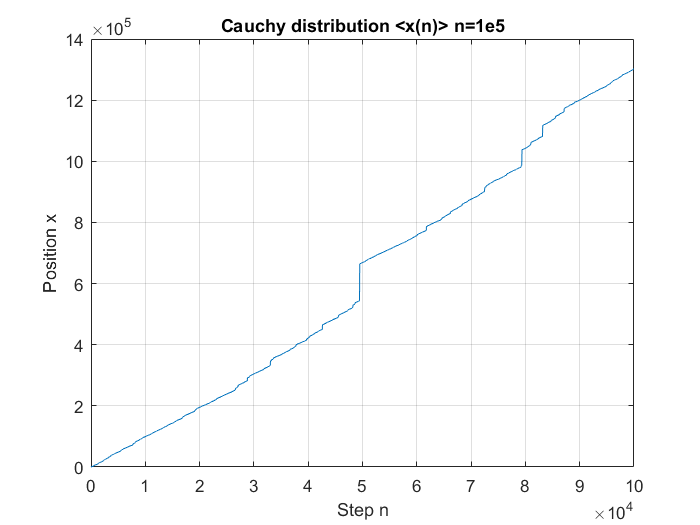
\includegraphics[width=0.9\linewidth]{./exercise2_1}
\caption{First order moment}
\label{fig:exercise2_1}
\end{figure}

\begin{lstlisting}
row = 1e3;column = 1e5;
G = zeros(row,column);
for kk=1:row
    Y = abs(cauc(b,column));
    for jj=2:column
        G(kk, jj) = Y(jj-1) + G(kk, jj-1);
    end
end
G_mean = mean(G,1);
s = @(x) x.*log(x);
t = [0:column-1];
figure;plot([0:column-1],G_mean)
title('Cauchy distribution <x(n)> n=1e5');xlabel('Step n');
ylabel('Position x');
\end{lstlisting}

As it is possible to see, the mean doesn't converge to a finite value.

\subsection{Scaling behaviour}
The cauchy distribution for the increment $y$ presents with a scaling behaviour for the average $\langle x(n) \rangle \sim n\mathrm{log}(n)$. This has a correspondent interpretation in the anomalous diffusion. The scaling relation is shown in Fig. (\ref{fig:exercise2_2}).


\begin{lstlisting}
figure;plot([0:column-1],G_mean, 'DisplayName','<x(n)>');
hold on;plot(t,s(t), '-r', 'DisplayName','nlog(n)')
title('Cauchy distribution - Scaling behaviour <x(n)> n=1e5');
xlabel('Step n');
ylabel('Position x');legend('show');
\end{lstlisting}

\begin{figure}
\centering
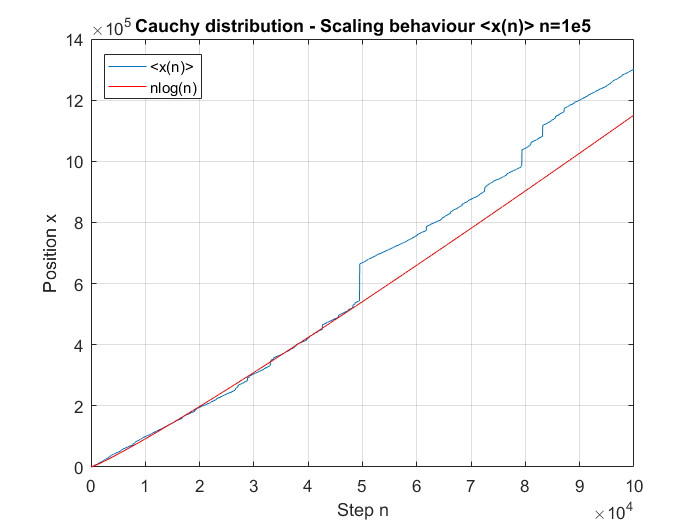
\includegraphics[width=0.9\linewidth]{./exercise2_2}
\caption{Scaling relation for a Cauchy process}
\label{fig:exercise2_2}
\end{figure}

\subsection{Convergence to Levy law for large n}
\subsubsection{$\mu$ = 1 - Cauchy process}
Let's define the normalized variable $u_n \equiv \frac{x_n}{n^{1/\mu}} = \frac{x_n}{n}$. We want to show that $P(u_n)$ for large n has a limit defined by $L(u)$:

\begin{equation}
L(u) = \frac{b}{u^{3/2}}exp(-\pi b^2/u)
\end{equation}

To do so, we consider M different realizations of a Cauchy process (M = 1000) and study the values $x_N^m$ of them, with N = 1e5, $m = 1,..., M$. Then, we divide $x_N^m$ by N and plot the histogram of the data (see Fig. (\ref{fig:exercise2_3})). As we see, the agreement between $L(u)$ and the histogram of the data is pretty good, even though there seems to be a \textit{shift} in the x-coordinate. This could be due to a non-perfect implementation of the Cauchy distribution in the following:

\begin{lstlisting}
function y = cauc(b,N)
    y = b*tan(0.5*pi*(rand(N,1)));
end
\end{lstlisting}

\begin{lstlisting}
L = @(x) x.^(-3/2).*exp(-pi./x);
GG = G(:,end)/(column);
edges = [0 1:0.5:50 51:2:100];
[nn, xx] = hist(GG, edges);
figure;
histogram(GG,edges, 'Normalization','probability', 'DisplayName', 'hist(u)');
hold on; plot([0:0.5:xx(end)],L([0:0.5:xx(end)]), '-r', 'DisplayName', 'Levy Function');
title('Convergence to Levy Function for \mu = 1');xlabel('u_n = x_n / n');
ylabel('Probability P(u)');legend('show');
hold on
\end{lstlisting}

\begin{figure}
\centering
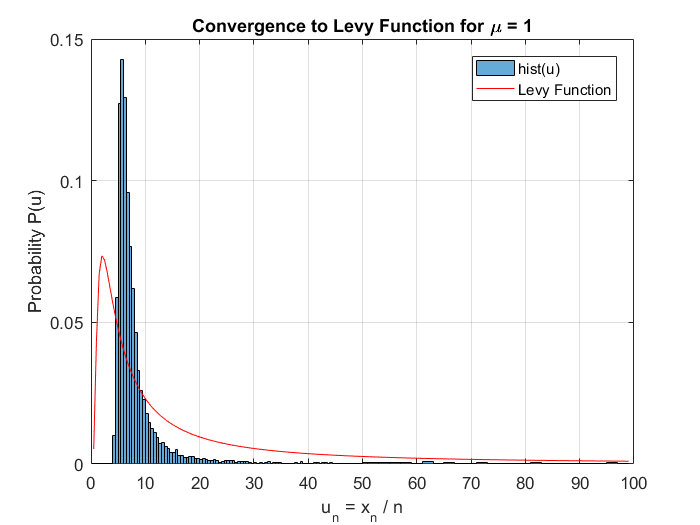
\includegraphics[width=0.9\linewidth]{./exercise2_3}
\caption{Convergence for mu = 1}
\label{fig:exercise2_3}
\end{figure}

\subsubsection{$\mu$ = 1/2}
To deal with this point, we used a "trick" that became clear after doing Exercise 3. It could be useful, then, to check the explanation given there.\\
By extracting random numbers from an exponential distribution, we can obtain a Levy probability distribution for any value of $\mu$ including 0.5. As we can see from Fig. (\ref{fig:levy}), also in this case the agreement between the Levy function and the histogram is extremely good, and without shifts of any sort as well (1e4 trajectories have been computed for 1e4 steps).

\begin{figure}
\centering
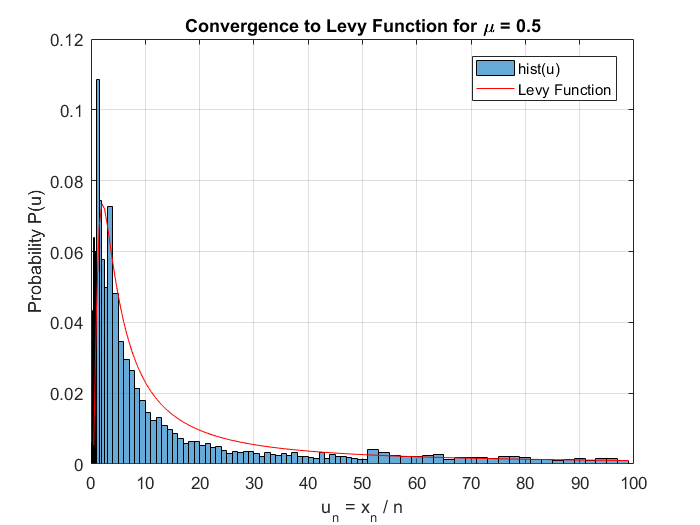
\includegraphics[width=0.9\linewidth]{./levy}
\caption{Convergence for mu = 0.5}
\label{fig:levy}
\end{figure}

Having read Exercise 3, the following code is self-explaining:
\begin{lstlisting}
pd=makedist('Exponential','mu',1);
row = 1e3;column = 1e5;
kT = 0.5;
b = 1;
G = zeros(row,column);
V = random(pd, row, column);tau=exp(V/kT);
for kk=1:row
    %Y = abs(cauc(b,column));
    for jj=2:column
        G(kk, jj) = tau(kk, jj-1) + G(kk, jj-1);
    end
end
G_mean = mean(G,1);
t = [0:column-1];
L = @(x) x.^(-3/2).*exp(-pi./x);
GG = G(:,end)/(column^2);
edges = [0:0.2:1 1:0.5:3 3:1:50 51:2:100];
[nn, xx] = hist(GG, edges);
figure;
histogram(GG,edges, 'Normalization','probability', 'DisplayName', 'hist(u)');
hold on; plot([0:0.5:xx(end)],L([0:0.5:xx(end)]), '-r', 'DisplayName', 'Levy Function');
title('Convergence to Levy Function for \mu = 0.5');xlabel('u_n = x_n / n');
ylabel('Probability P(u)');legend('show');
hold on
\end{lstlisting}


\newpage
\section{Arrhenius cascade}
In this section we present the plots commented on the hand-typed paper. Additionally, we attach the code used in generating random numbers from a given distribution.

\begin{figure}
\centering
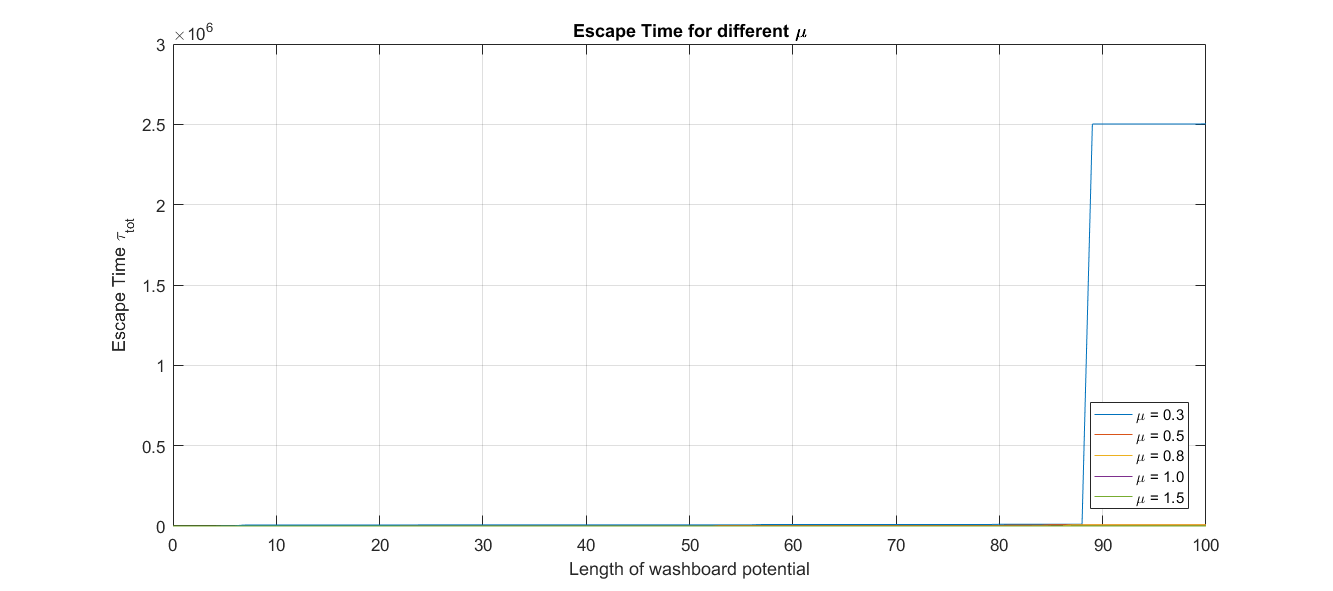
\includegraphics[width=0.9\linewidth]{./escape_time1}
\caption{Comparison of the escape times for different values of mu}
\label{fig:escape_time1}
\end{figure}

\begin{figure}
\centering
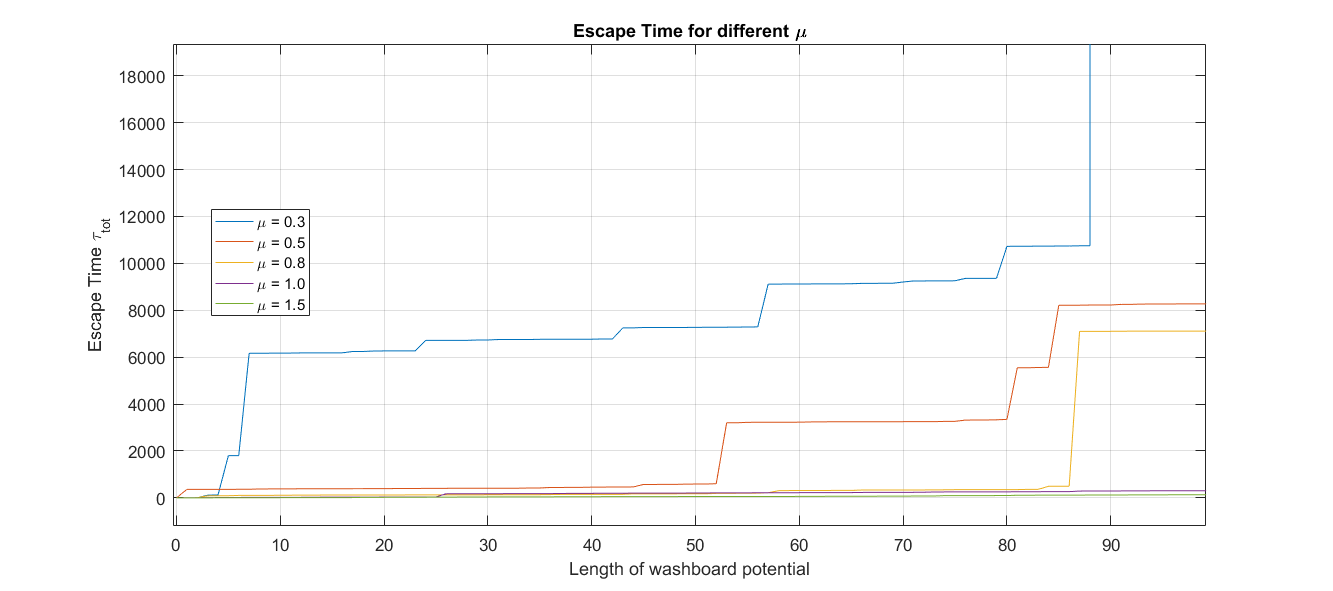
\includegraphics[width=0.9\linewidth]{./escape_time2}
\caption{Comparison of the escape times for different values of mu - zoom}
\label{fig:escape_time2}
\end{figure}

\begin{figure}
\centering
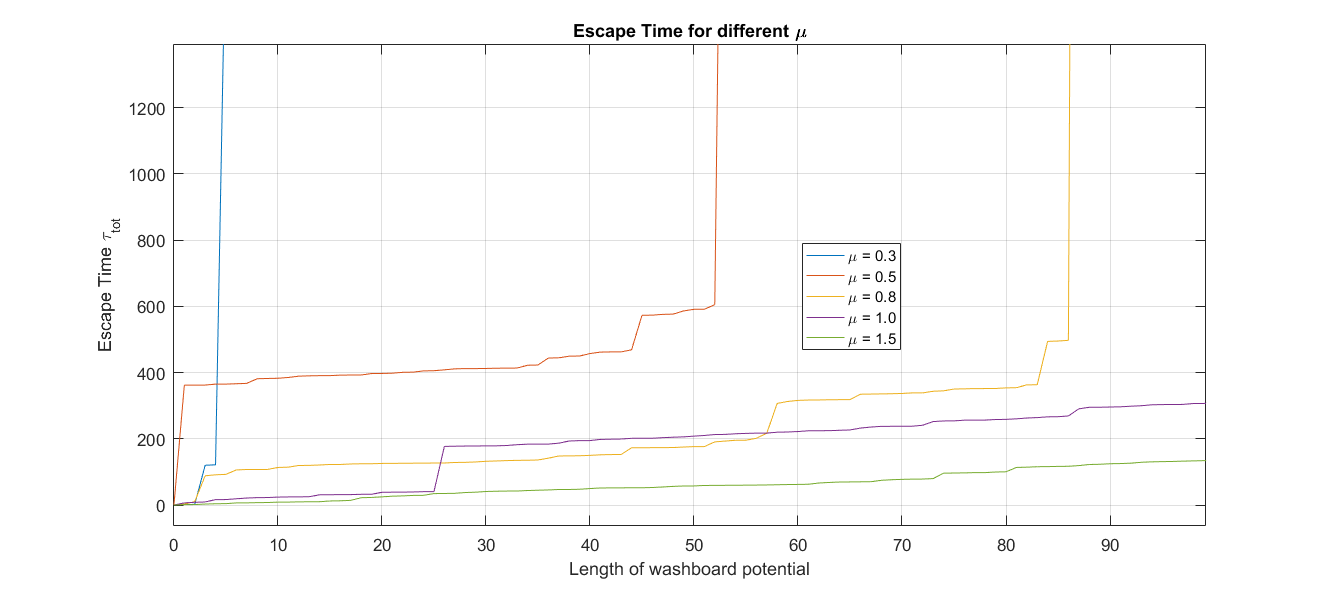
\includegraphics[width=0.9\linewidth]{./escape_time3}
\caption{Comparison of the escape times for different values of mu - zoom}
\label{fig:escape_time3}
\end{figure}

\begin{figure}
\centering
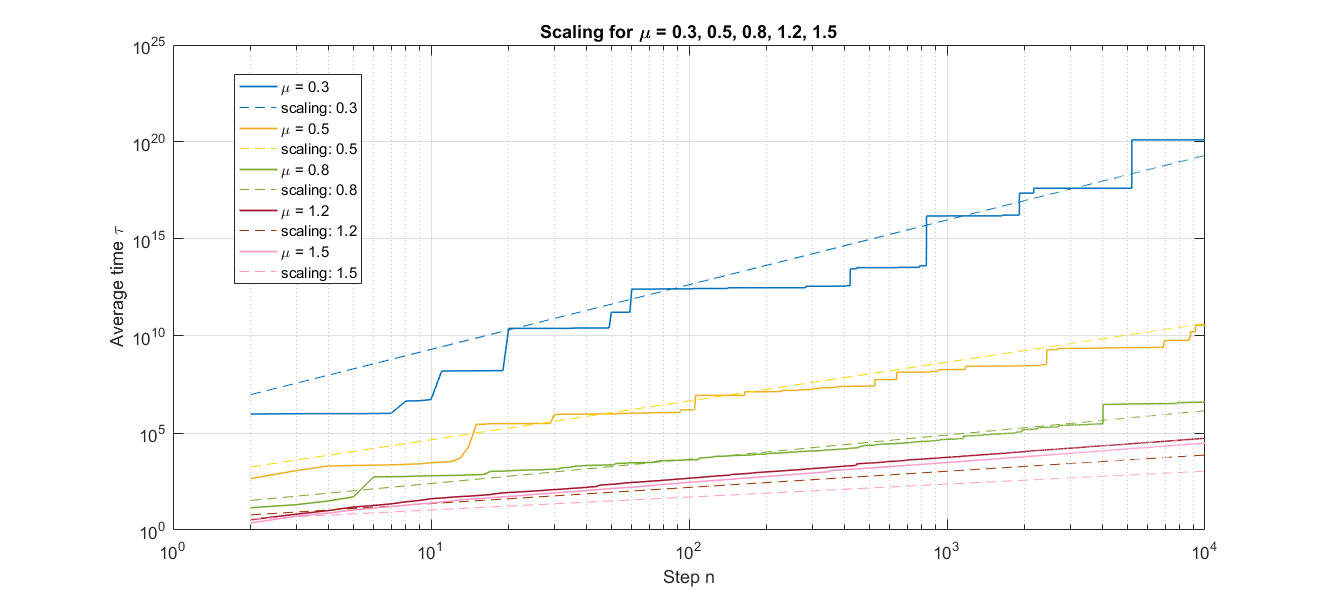
\includegraphics[width=0.9\linewidth]{./exercise3_2}
\caption{Scaling for different mu}
\label{fig:exercise3_2}
\end{figure}

\begin{figure}
\centering
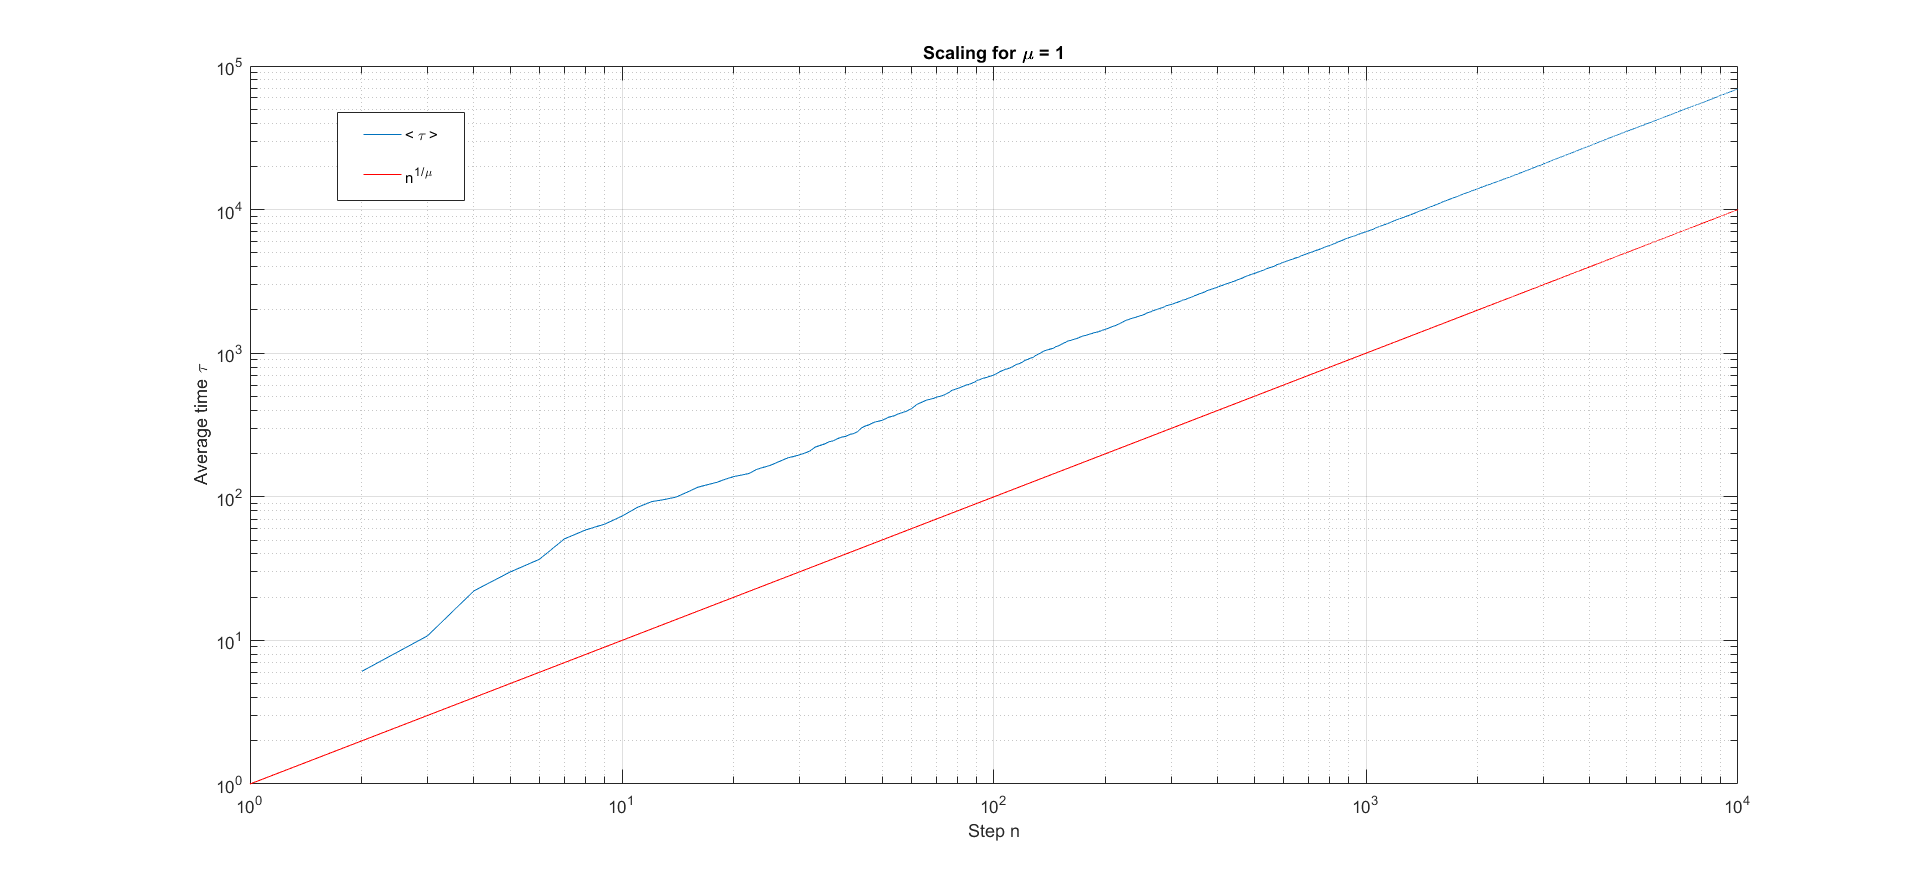
\includegraphics[width=0.9\linewidth]{./exercise3_3}
\caption{Scaling for mu = 1}
\label{fig:exercise3_3}
\end{figure}


\begin{lstlisting}
	mu = mu_array(ss);    
    p = @(x) (mu./(mu^2 + x.^(1+mu))).*heaviside(x);
    norma = integral(p, 0, Inf);
    p = @(x) ((mu./(mu^2 + x.^(1+mu))).*heaviside(x))/norma;
    cum_int = @(y) integral(p,0,y);    
    N = 1e3;
    Nrand = 100;
    rn = rand(Nrand,1);
    position = zeros(Nrand,1);
    for jj=1:Nrand
        disp(jj)
        step = 0;
        a = -2;b = 7;
        counter = 0;
        while step == 0 && counter < 100;
        %here we create a grid both on the x-axis 
        %and on the correspondent image of the CDF
            x = logspace(a,b,N);
            I = zeros(N,1);
            for kk=1:N
                I(kk) = cum_int(x(kk));
            end
            %we want the last value of x which is smaller than CDF^-1(rand)
            id = find(I <rn(jj));
            %check if the extremal value of x is too small
            if ~isempty(id)
                id = id(end);
                %check if the minimal value of x is too large
                if ~(id == N)
                    z1 = x(id);z2 = x(id+1);
                    if (rn(jj) - I(id)) <= 1e-2
                        step = z1;
                    else
                        a = log10(z1);b = log10(z2);
                            %t = logspace(log10(z1),log10(z2),1e5);
                    end
                else
                    z1 = x(end);z2 = x(end)*100;
                    a = log10(z1);b = log10(z2);
                end
            else
                z1 = x(1)/100;z2 = x(1);
                a = log10(z1);b = log10(z2);
            end
             counter = counter + 1;
        end
        position(jj) = step;
    end
    for mm=2:Nrand
        position(mm) = position(mm)+position(mm-1);
    end
    position = [0 position']';    
    plot([0:Nrand], position, '-', 'DisplayName', ['\mu = ', sprintf('%1.1f',mu)]);
    hold on  
\end{lstlisting}

\end{document}